\section{eo\-Quad\-Distance$<$ EOT $>$ Class Template Reference}
\label{classeo_quad_distance}\index{eoQuadDistance@{eoQuadDistance}}
This is a generic class for Euclidain distance (L2 norm) computation: assumes the 2 things are std::vectors of something that is double-castable.  


{\tt \#include $<$eo\-Distance.h$>$}

Inheritance diagram for eo\-Quad\-Distance$<$ EOT $>$::\begin{figure}[H]
\begin{center}
\leavevmode
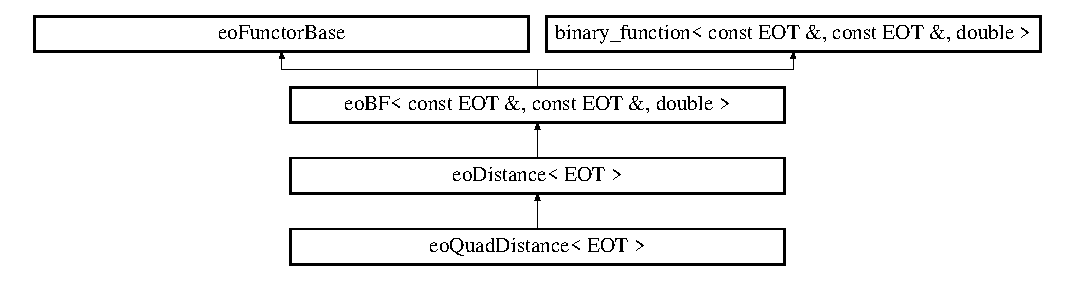
\includegraphics[height=3.33333cm]{classeo_quad_distance}
\end{center}
\end{figure}
\subsection*{Public Member Functions}
\begin{CompactItemize}
\item 
double {\bf operator()} (const {\bf EOT} \&\_\-v1, const {\bf EOT} \&\_\-v2)\label{classeo_quad_distance_a0}

\begin{CompactList}\small\item\em The pure virtual function that needs to be implemented by the subclass. \item\end{CompactList}\end{CompactItemize}


\subsection{Detailed Description}
\subsubsection*{template$<$class EOT$>$ class eo\-Quad\-Distance$<$ EOT $>$}

This is a generic class for Euclidain distance (L2 norm) computation: assumes the 2 things are std::vectors of something that is double-castable. 



Definition at line 44 of file eo\-Distance.h.

The documentation for this class was generated from the following file:\begin{CompactItemize}
\item 
eo\-Distance.h\end{CompactItemize}
